\documentclass[a4paper]{article}

\usepackage[english]{babel}
\usepackage{amsmath}
\usepackage{float}
\usepackage{amssymb}
\usepackage{dsfont}
\usepackage{graphicx}
\usepackage{listings}
\usepackage[hyphens]{url}
\usepackage{titling}
\usepackage{varwidth}
\usepackage{hyperref}
\usepackage{url}
\usepackage{adjustbox}
\usepackage{color} %red, green, blue, yellow, cyan, magenta, black, white
\definecolor{mygreen}{RGB}{28,172,0} % color values Red, Green, Blue
\definecolor{mylilas}{RGB}{170,55,241}


\usepackage{geometry}
 \geometry{
 a4paper,
 total={165mm,257mm},
 left=20mm,
 top=20mm,
 }

\title{Natural Computing\\Assignment 5}
\author{
  Christoph Schmidl\\ s4226887\\      \texttt{c.schmidl@student.ru.nl}
  \and
  Koen Vijverberg\\ s4132858\\     \texttt{koen.vijverberg@student.ru.nl}
  \and
  Alex Kolmus\\	s4125304\\	\texttt{alex.kolmus@student.ru.nl}
}
\date{\today}

\begin{document}
\maketitle


\subsection*{Exercises on Convolutional Neural Networks}

\begin{enumerate}

	% Task 1	
	\item Consider a convolutional neural network (CNN) with one-dimensional (1D) input. While two dimensional (2D) CNNs can be used for example for grayscale images, one-dimensional CNNs could be used for time-series such as temperature or humidity readings. Concepts for the 1D-case are equivalent to 2D networks.\\
	We interpret data in our network as three-dimensional array where a row denotes a feature map (also called filter, kernel), a column denotes a single dimension of the observation, and the depth of the array represents different observations. As we will only work with single input vector, the depth will always be one. Let the following CNN be given:
	
	\begin{itemize}
		\item Input $I$: Matrix of size 1 x 12 x 1. We therefore have an input with twelve dimensions consisting of a single feature map.
		\item First convolutional layer with filters $F_0^1 = (-1, 0, 1)$ and $F_1^1 = (1,0,-1)$ that generates two output feature maps from a single input feature map. Use \textit{valid} mode for convolutions. Mode \textit{valid} returns output of length max(M,N) - min(M,N) + 1, where M is the size of the array and N = 3 is the size of the filter. The convolution product is only given for points where the signals overlap completely. Values outside the signal boundary have no effect.
		\item Max-pooling layer with stride 2 and filter size 2. Note that max-pooling pools each feature map separately.
		\item Convolutional layer with convolutional kernel $F_0^2 = (-1,0,1), (1,0,-1)$ of size 2 x 3 x 1.
		\item Fully connected layer that maps all inputs to two outputs. The first output is calculated as the negative sum of all its inputs, and the second layer is calculated as the positive sum of all its inputs.
		\item Sigmoidal activation function
	\end{itemize}
	
\begin{enumerate}
	% Task 1a)
	\item Draw the network.\\
	\textbf{Solution:}\\
	
	On the left side are the expected data dims, on the right side the operations performed.
	\begin{figure}[H]
	\centering
  	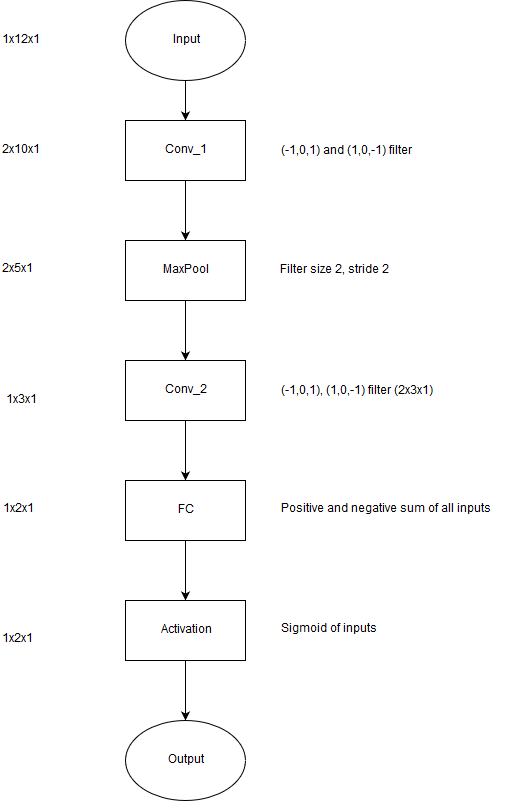
\includegraphics[width=0.7\textwidth]{images/CNN_ex_1.png}
	\end{figure}
	
	
	
	
	\item Calculate the response of the CNN for the two inputs (0;0;0;0;1;1;1;1;0;0;0;0) and (1;1;1;1;0;0;0;0;1;1;1;1).\\
	\textbf{Solution:}\\ \\
	Filter sizes are applied in order mentioned in the exercise. For the fully-connected (FC) layer the positive sum is computed first.
	\begin{center}
    \begin{tabular}{| l | p{5cm} |}
    \hline
    Input & (0;0;0;0;1;1;1;1;0;0;0;0) \\ \hline
    Conv\_1: & (0;0;1;1;0;0;-1;-1;0;0) \newline (0;0;-1;-1;0;0;1;1;0;0) \\ \hline
    MaxPool: & (0;1;0;-1;0) \newline (0;-1;0;1;0) \\ \hline
    Conv\_2: & (0;-4;0) \\ \hline
	FC: & (-4;4) \\ \hline
	Activation: & (0.018;0.982) \\ \hline
    \end{tabular}
    \end{center}
    \begin{center}
    \begin{tabular}{| l | p{5cm} |}
    \hline
    Input & (1;1;1;1;0;0;0;0;1;1;1;1) \\ \hline
    Conv\_1: & (0;0;-1;-1;0;0;1;1;0;0) \newline (0;0;1;1;0;0;-1;-1;0;0) \\ \hline
    MaxPool: & (0;-1;0;1;0) \newline (0;1;0;-1;0) \\ \hline
    Conv\_2: & (0;4;0) \\ \hline
	FC: & (4;-4) \\ \hline
	Activation: & (0.982;0.018) \\ \hline
    \end{tabular}
    \end{center}
	
\end{enumerate}	

% Task 2
\item Convolutional Networks in practice. To start:

\begin{itemize}
	\item download and extract the archive 'assignment\_cnn.tar.gz' from blackboard;
	\item follow the instructions inside the 'README.txt'
\end{itemize}

If you are unable to successfully setup your environment and run the ipython notebook then you can download the virtualbox image (hosted here: \url{https://surfdrive.surf.nl/files/index.php/s/EMYHsFb8X7mk11V}) where everythin is already configures.\\
Consider the practical assignment of:

\begin{enumerate}
	% Task 2a)
	\item implementing layers of a CNN (ConvolutionalNeuralNetworks.ipynb)\\
	\textbf{Solution:}\\
	See submitted archive file.
	
	
	% Task 2b)
	\item modifying a simple architecture of a CNN to achieve higher accuracy on the MNIST dataset (mnist.ipynb)\\
	\textbf{Solution:}\\
	See submitted archive file
	
\end{enumerate}
	
\end{enumerate}
\end{document}